\subsubsection{Yule-Walker (YW) Method for frequency estimation}
\textbf{Multicomponent sinusoidal signal in AWGN}
\begin{align*}
X(t) &= s(t) + W(t), \qquad t \in [0,T] \\[4pt]
s(t) &= \sum_{k=1}^{K} A_k \cos\!\bigl(2\pi f_k t + \theta_k\bigr),
\quad \text{with } f_k T \gg 1, \quad W(t) \sim \text{AWGN}, \qquad S_W(f) = \frac{N_0}{2}.
\end{align*}
\begin{itemize}
    \item Since the poles of the AR(P) model determine the peaks in the spectrum, we can estimate the frequencies of a \textbf{multicomponent sinusoidal signal} in AWGN by estimating the location of the \(K\) highest peaks in the (estimated) PSD. The estimates of the \(K\) frequencies are obtained from the phases of teh \(K\) poles (with positive angle) closest to the unit circle (\underline{\textbf{YW method}}):
\begin{align*}
\hat{f}_k = \frac{1}{2\pi} \angle p_k, 
\qquad k = 1,2,\dots,K
\end{align*}

    \item Once we have estimated the frequencies, amplitudes and phases can be estimated in the usual way from the modulo and phase of the data vector Fourier Transform at the estimated frequencies.
\begin{figure}[H]
        \centering
        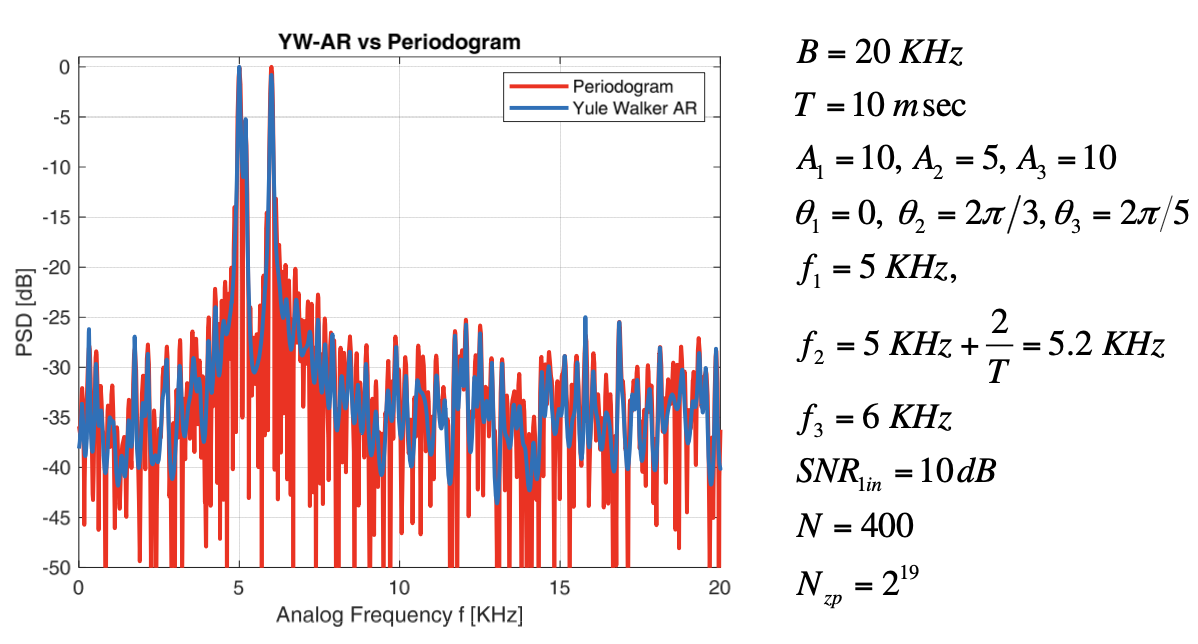
\includegraphics[width=0.65\linewidth]{Image/pdf 6/67.PSD_YW.png}
        \label{fig:placeholder}
    \end{figure}
\begin{figure}[H]
    \centering
    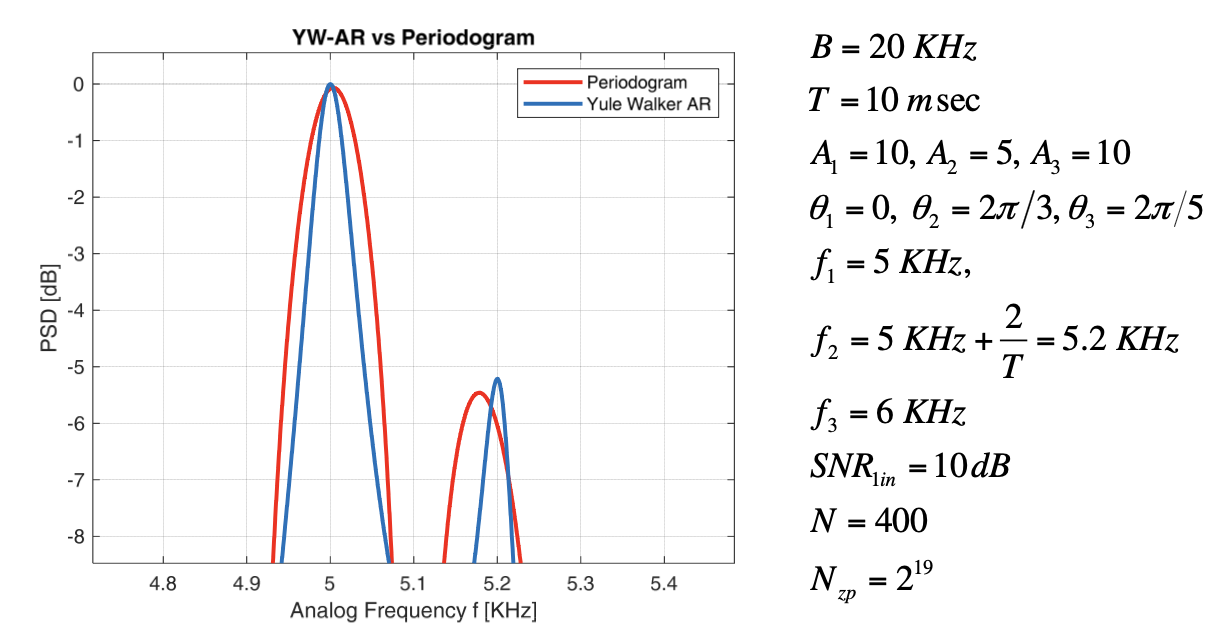
\includegraphics[width=0.65\linewidth]{Image/pdf 6/68.YW_periodo.png}
    \label{fig:placeholder}
\end{figure}
\begin{figure}[H]
    \centering
    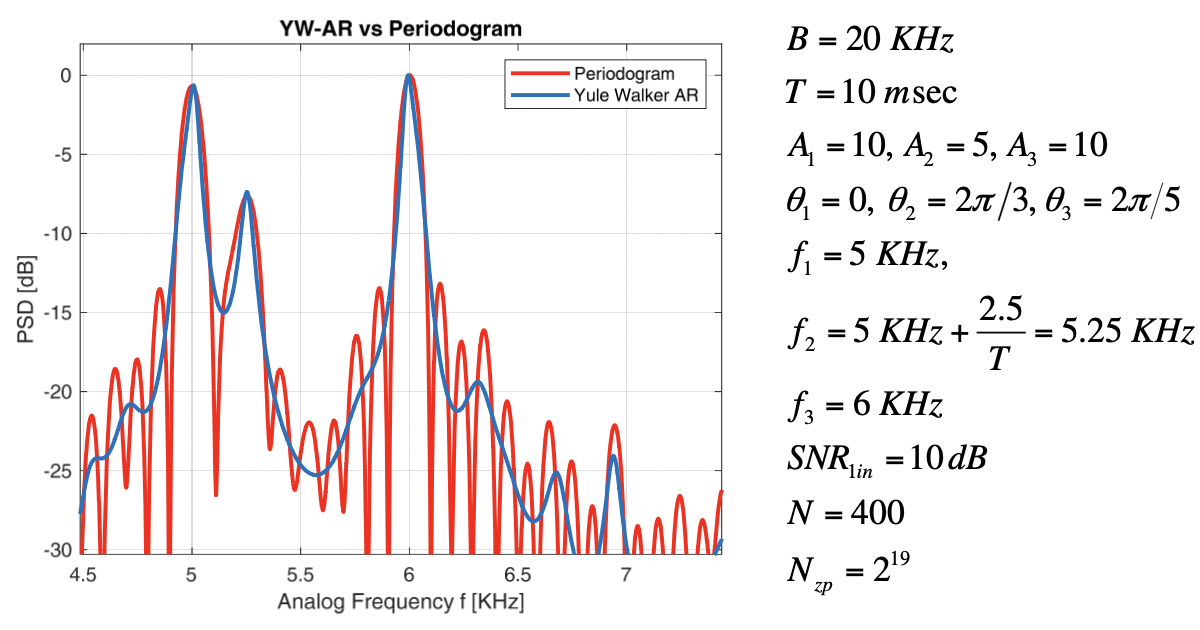
\includegraphics[width=0.65\linewidth]{Image/pdf 6/69.YW_20.png}
    \label{fig:placeholder}
\end{figure}
\begin{figure}[H]
    \centering
    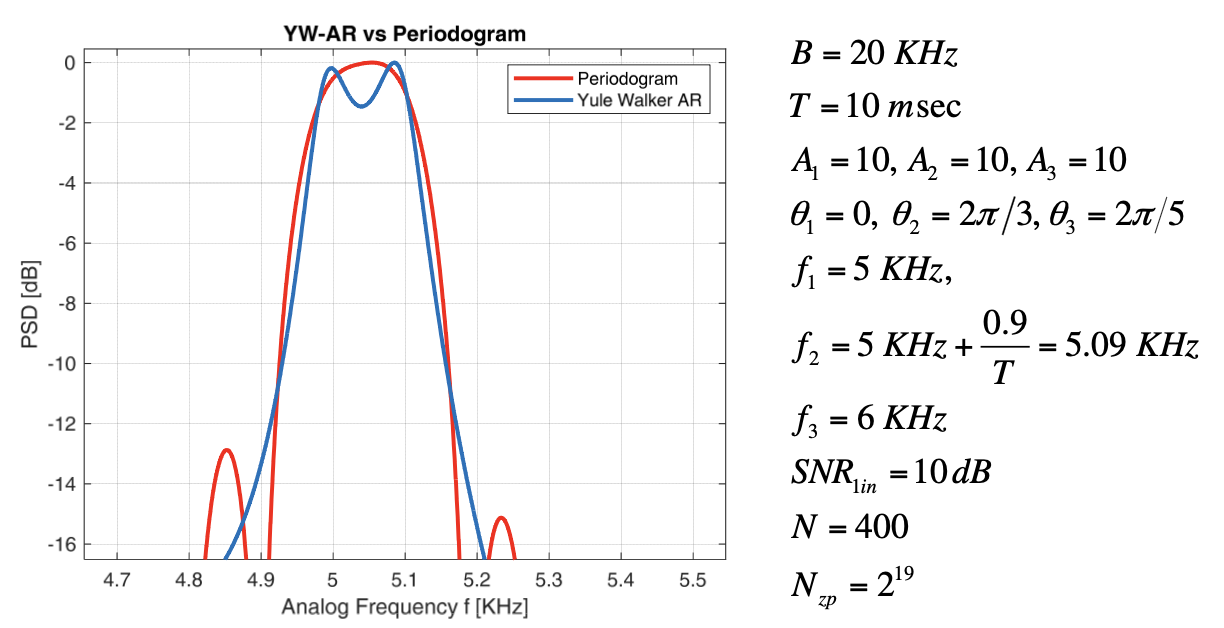
\includegraphics[width=0.65\linewidth]{Image/pdf 6/70.YW_Periodo_2.png}
    \label{fig:placeholder}
\end{figure}
\item \textbf{YW-AR is a superresolution method to estimate the frequencies of a multicomponent sinusoidal signal in AWGN}

\end{itemize}
\subsection{SUMMARY}
\begin{itemize}
    \item The \textbf{ARMA(P,Q) model identification} problem consists in the estimation of the unknown parameters \textbf{a,b} and the power of the innovation procecss \(W[n]\) of the ARMA model that better fits the estimated ACF sequence, having available N samples of a realization of the process \(X[n]\):
\begin{align*}
\{X[n]\}_{n=0}^{N-1}
&\quad\Rightarrow\quad
\{\hat{R}_X[m]\}_{m=0}^{Q+P}
\quad\Rightarrow\quad
\{\hat{\sigma}_w^{2}, \hat{\mathbf{a}}, \hat{\mathbf{b}}\}
\quad\Rightarrow\quad
\hat{S}_X\!\left(e^{j 2\pi f}\right)
\end{align*}

    \item For \textbf{AR(P) processes, model identification} requires the solution of a system of \(P+1\) \underline{\textbf{linear}} equations, that can be solved efficiently by using the Levinson-Durbin algorithm or the Shur algorithm.
    \item The system of equations to be solved to estimate the vector \textbf{b} for MA(Q) or ARMA(P,Q) processes is instead \underline{\textbf{non-linear}}.
    \item The \textbf{Model order selection(MOS)} problem is not treated here.

    \item The most important methods to estimates the parameters of an ARMA(P,Q) process,  given P and Q are:
    \begin{itemize}
        \item \textbf{Modified Yule-Walker Method (Matlab: mywarma.m)}
        \item \textbf{Two-Stage least-Squares method (Matlab: isarma.m)}
    \end{itemize}
\end{itemize}

\clearpage